
\fullcite{beps10}

\begin{multicols}{2}
\begin{center}
{\bf Article excerpts}
\\ 
{\bf Notes and remarks}
\end{center}
\end{multicols}

%------------------------------------------------------------------------------

\begin{multicols}{2}
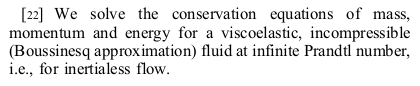
\includegraphics[width=8.3cm]{images/viscoelasticity/beps10a}\\
Incompressible ! Boussinesq approximation.
\end{multicols}

\begin{multicols}{2}
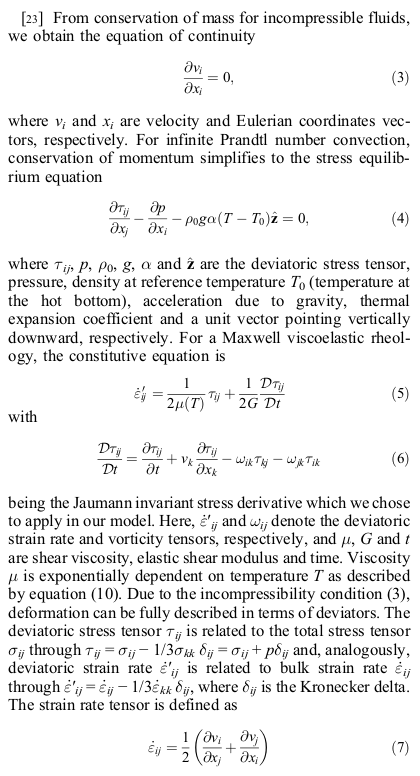
\includegraphics[width=8.3cm]{images/viscoelasticity/beps10b}\\
\[
\vec\nabla\cdot \vec\upnu=0
\]
\[
\dot\varepsilon_{ij}^d = \frac{1}{2\eta} \tau_{ij} + \frac{1}{2\mu} \frac{{\cal D}\tau_{ij}}{{\cal D}t}
\]
with
\[
\frac{{\cal D}\tau_{ij}}{{\cal D}t} =  \frac{\partial \tau_{ij}}{\partial t} 
+ \upnu_k \frac{\partial \tau_{ij}}{\partial x_k}
- (\dot{\omega}_{ik}\tau_{kj} - \tau_{jk} \dot{\omega}_{ik} ) 
\]

Note that Eq 6 is formulated with two minus signs. At first glance one could
think it is a mistake/typo, but since $\omega$ is anti-symmetric
the last term is then 
$\omega_{jk}\tau_{ik} = -\omega_{kj}\tau_{ik} = -\tau_{ik} \omega_{kj} = -{\bm\tau}\cdot\dot{\bm\omega} $

\end{multicols}

\begin{multicols}{2}
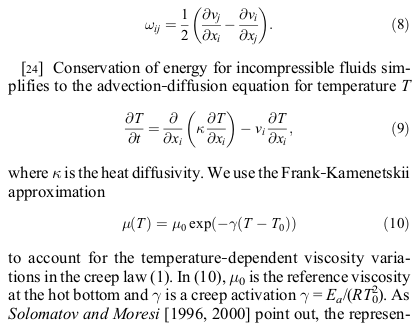
\includegraphics[width=8.3cm]{images/viscoelasticity/beps10c}
\end{multicols}



